\documentclass[11pt a4paper]{article}
\usepackage[margin=2cm]{geometry}
\usepackage{amsmath, amssymb}
\usepackage{graphicx}
\usepackage{float}
\usepackage{aligned-overset}
\usepackage{subcaption}
\usepackage{tabularx} % fuer gleichungen nebeneinander

% partielle ableitungen
\newcommand{\delr}{\partial_r}
\newcommand{\deltheta}{\partial_\theta}
\newcommand{\delphi}{\partial_\varphi}

% elektrische feldkonstante
\newcommand{\epsz}{\epsilon_0}
% 1 / 4pi eps
\newcommand{\kco}{\frac{1}{4\pi\epsilon_0}}

% rotation
\newcommand{\rot}{\text{rot}}

% fancy header
\usepackage{fancyhdr}
\fancyhf{}
% vspaces in den headern fuer Distanzen notwendig
% linke Seite: Namen der Abgabegruppe
\lhead{\textbf{Matthias Maile\\Roman Surma}\vspace{1.5cm}}
% rechte Seite: Modul, Gruppe, Semester
\rhead{\textbf{Physik II - Gruppe 2\\Sommersemester 2020}\vspace{1.5cm}}
% Center: nr. des blattes
\chead{\vspace{2.5cm}\huge{\textbf{19. Übungsblatt}}}
% benoetigt damit der eigentliche Text nicht in der Überschrift steckt
\setlength{\headheight}{4cm}

% zum zeichnen tikz
\usepackage{tikz}

% fuer fabigen text
\usepackage{xcolor}

% irgendwas mit figures
\usepackage{subcaption}

\begin{document}
\thispagestyle{fancy}
\section*{Aufgabe 1}
a) Das elektrische Feld im Bereich des Kondensators folgt aus einem 
Wegintegral:
\[
	E = \frac{\sigma}{\epsz}, \quad U = - \int_0^d E \ dl
	\Rightarrow
	U = \frac{-\sigma \ d}{\epsz} \Rightarrow
	E = \frac{-U}{d} \tag{1.1}
\]
Die gesamte Kraft auf ein geladenes Teilchen in einem magnetischen 
und elektrischen Feld ist gegeben durch:
\[ \vec F_\text{ges} = q (\vec E + \vec v \times \vec B) \]
Das stellen wir zu $v$ um:
\begin{align*}
	\vec F_\text{ges} = q (\vec E + \vec v \times \vec B) 
	\overset{!}&{=} \vec 0 \\
	% keine vektoren schreibweise, q kuerzen
	E &= vB \\
	v &= \frac{E}{B} \\
	% 1.1 einsetzen
	(1.1) \Rightarrow v &= \frac{U}{d \cdot B} 
	% ergebnis
	\approx \frac23 c
\end{align*}

\begin{figure}[H]
	\centering
	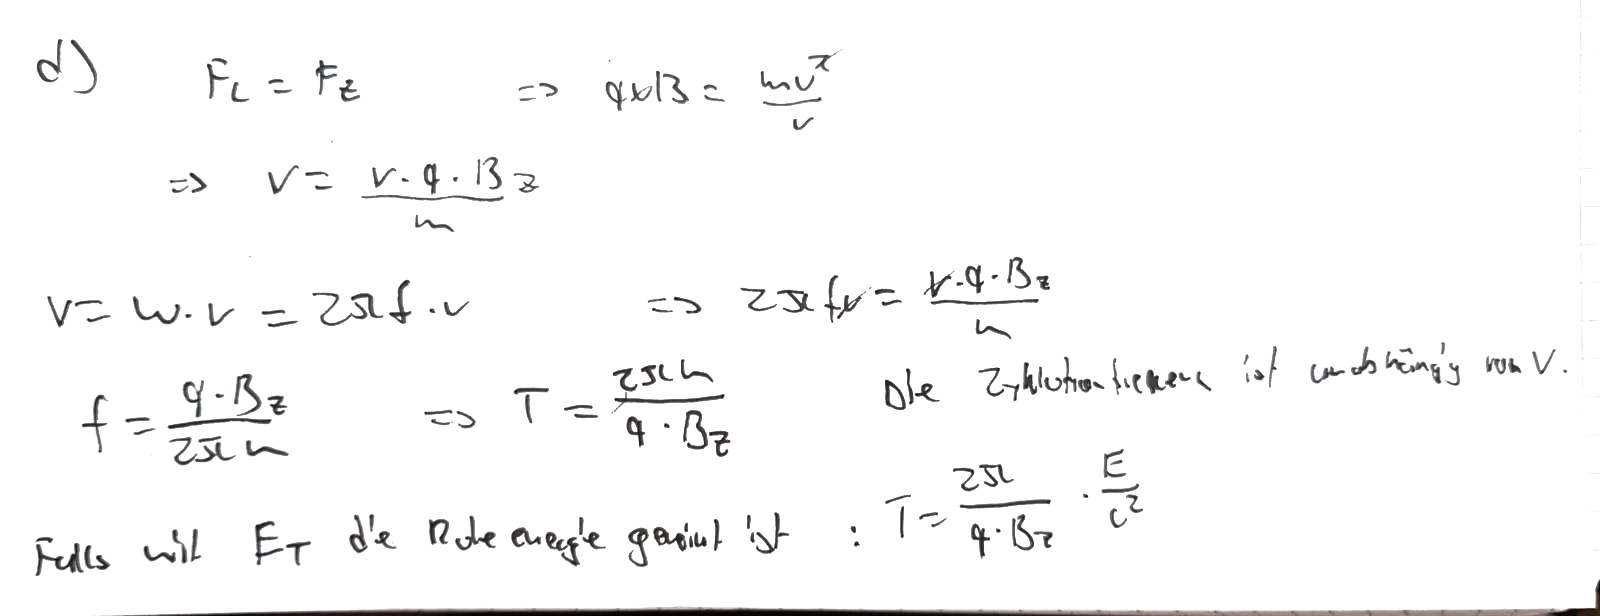
\includegraphics[width=15cm]{1d.jpg}
\end{figure}

\vspace{0.5cm}
e) Im Zyklotron werden die Teilchen "nach links" abgelenkt (in 
Bewegungsrichtung betrachtet). Obwohl im Bereich des Kondensator die 
Richtung des magnetischen Feldes die gleiche ist, werden die Teilchen in 
die andere Richtung gelenkt.

\newpage
\setlength{\headheight}{0cm}

\begin{figure}[H]
	\centering
	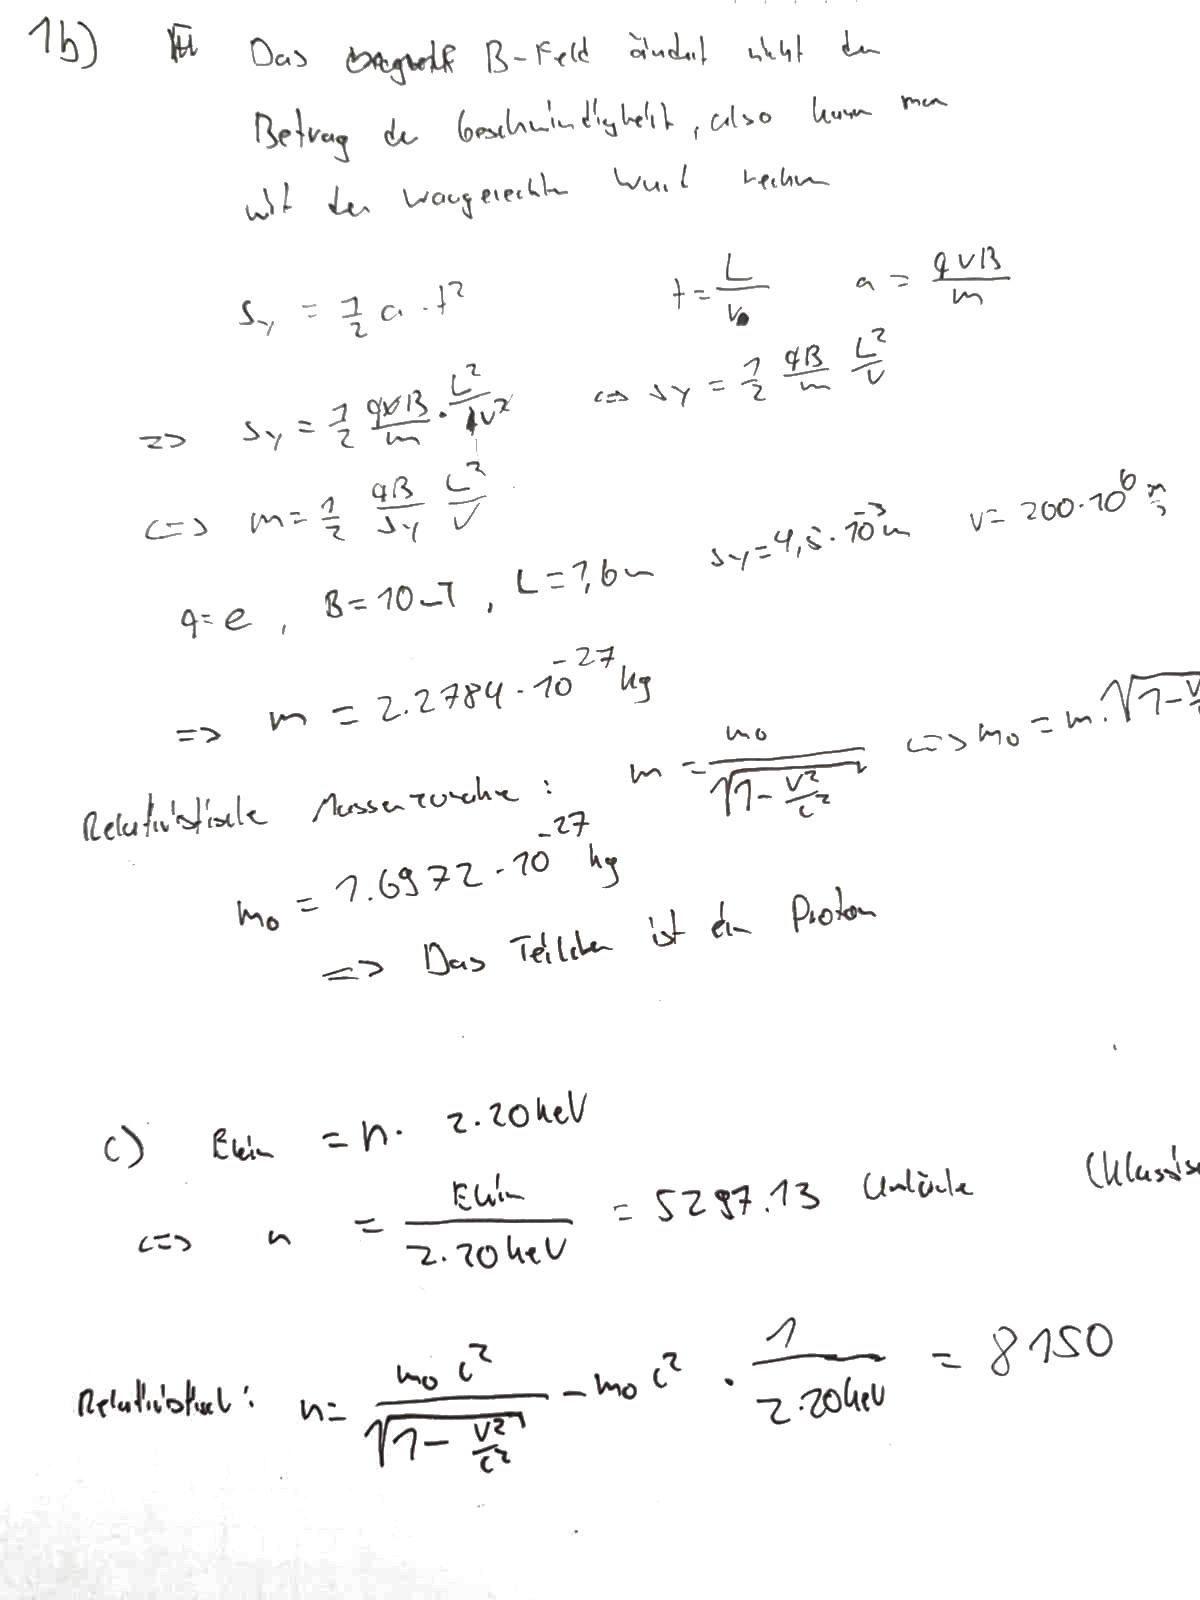
\includegraphics[width=15cm]{1bc.jpg}
\end{figure}

\newpage
\setlength{\headheight}{0cm}

\section*{Aufgabe 2}
a)
\begin{enumerate}
	\item[(i)] 
		$ \epsilon_{ijk} 
		= \alpha \ \epsilon_{jki} 
		= \alpha \ \epsilon_{ijk}
		\Rightarrow \alpha = 1$
	\item[(ii)]
		$ \epsilon_{ijk} 
		= \alpha \ \epsilon_{jik} 
		= -\alpha \ \epsilon_{ijk}
		\Rightarrow \alpha = -1$
	\item[(iii)]
		$ \epsilon_{iik} 
		= \alpha \ \epsilon_{ijk} 
		= 0
		\Rightarrow \alpha = 0$
\end{enumerate}
\vspace{0.5cm}
b) Zur besseren Lesbarkeit wird Einsteinsche Summenkonvention verwendet.
\begin{enumerate}
	\item[(i)]
		$ \epsilon_{ijk} \ \epsilon_{ijk} = \epsilon_{ijk}^2
		= \begin{cases} 
			1 & \text{für Permutationen von 1,2,3} \\
			0 & \text{sonst}
		\end{cases} $
	\item[(ii)]
		$ \epsilon_{ijk} \ \epsilon_{kmn} =
		\begin{cases}
			1 & \text{für }  i=m \wedge j=n \\
			-1 & \text{für } i=n \wedge j=m \\
			0 & \text{sonst} 
		\end{cases} $
\end{enumerate}
\vspace{0.5cm}
c)
\begin{align*}
	\vec a \times (\vec b \times \vec c)
	% aeusseres kreuzprodukt in indize schreibweise
	&= \epsilon_{ijk} \ \hat i \cdot a_j \cdot (\vec b \times \vec c)_k
	\\
	% inneres kreuzprodukt in indizesnotation
	&= \epsilon_{ijk} \ \hat i \cdot a_j \cdot 
	\epsilon_{kmn} \cdot b_m \cdot c_n
	\\
	% ergebnis aus b) (ii) einsetzen
	b)(ii) \Rightarrow
	&= \hat i \cdot b_i a_j c_j - \hat i \cdot c_i a_j b_j
	\\
	% \hat i und b_i bzw c_i zu vektoren umformen
	&= \vec b \cdot a_j c_j - \vec c \cdot  a_j b_j
	\\
	% a c skalarprodukt erzeugen
	&= \vec b \ (\vec a \cdot \vec c) - \vec c \ (\vec a \cdot \vec b)
	\\
\end{align*}

\newpage
\section*{Aufgabe 3}
a) Für die Konfiguration der Richtung von $E$- und $B$-Feld existieren zwei
Möglichkeiten:
\begin{figure}[H]
	\centering
	\begin{subfigure}[b]{0.3\textwidth}
		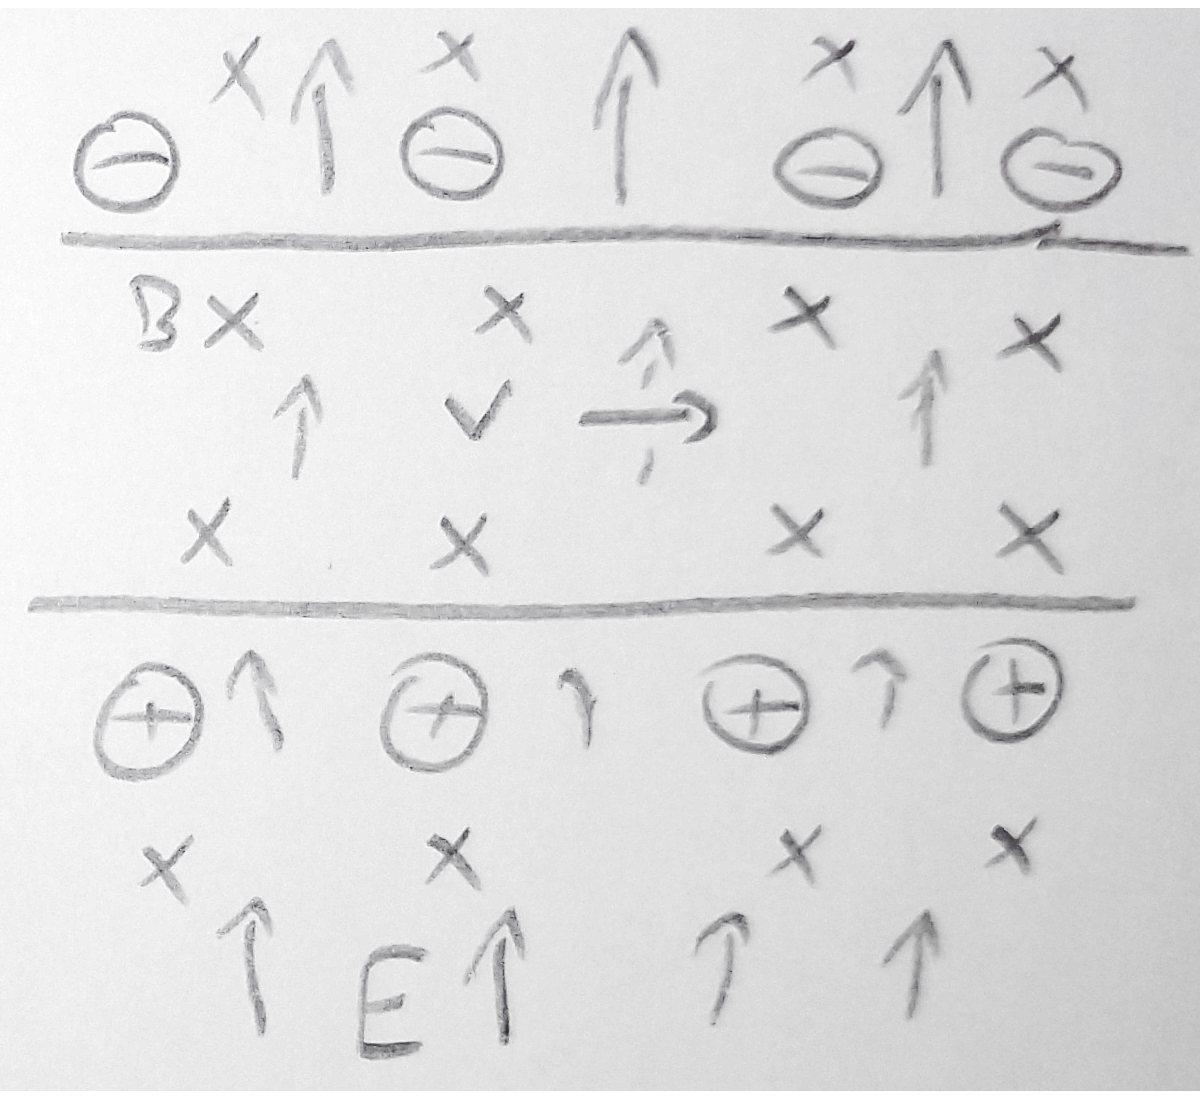
\includegraphics[width=\textwidth]
		{aufgabe3a_efeld_oben.png}
		\caption{E-Feld nach oben gerichtet,\\B-Feld ``zum Leser``}
	\end{subfigure}
	~
	\begin{subfigure}[b]{0.3\textwidth}
		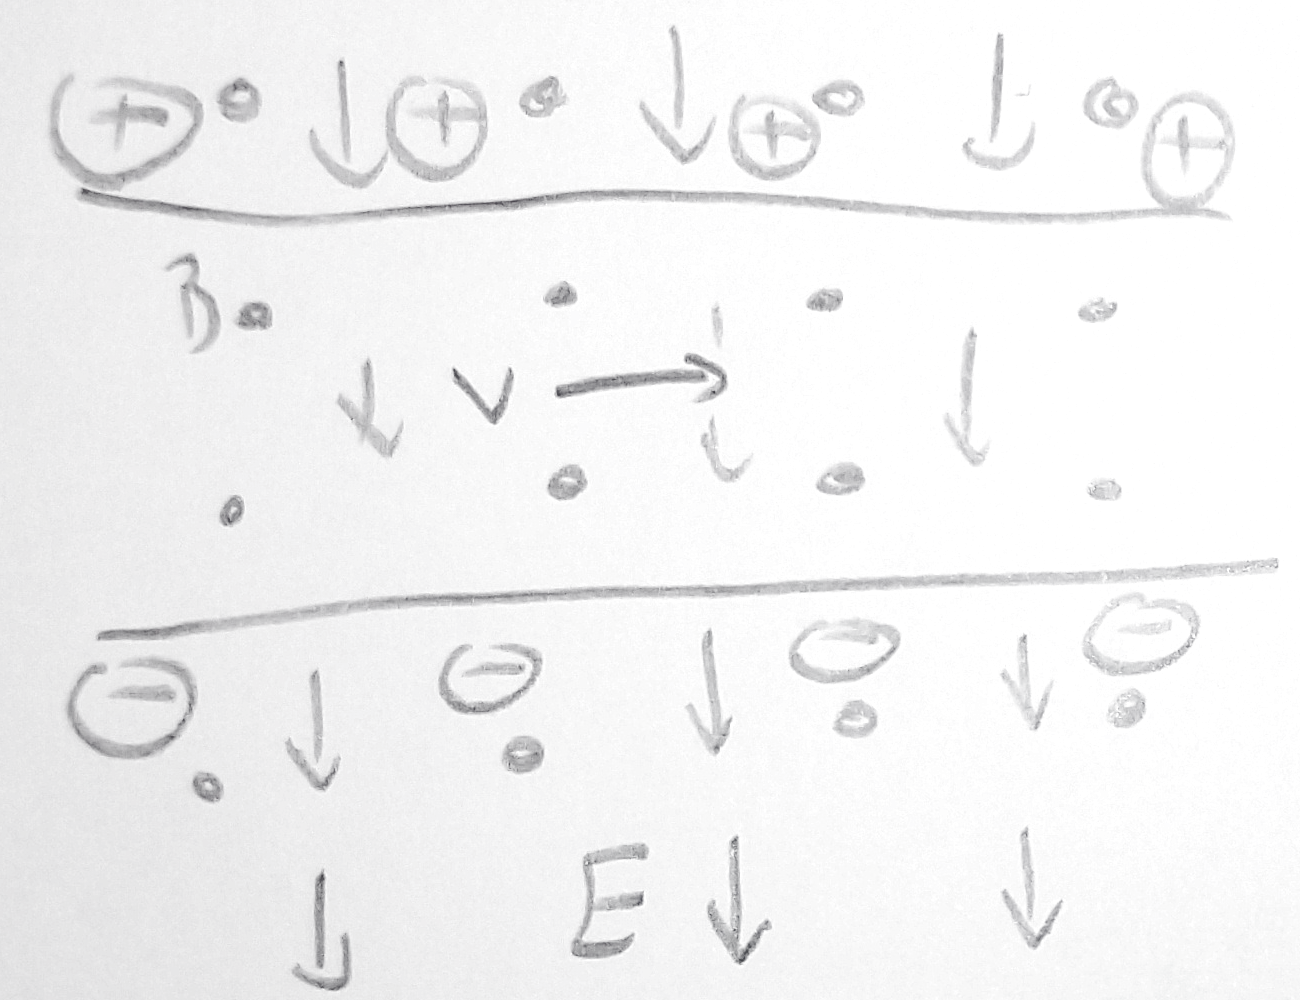
\includegraphics[width=\textwidth]
		{aufgabe3a_efeld_unten.png}
		\caption{E-Feld nach unten gerichtet,\\B-Feld ``ins Papier``}
	\end{subfigure}
\end{figure}
Da das $E$-Feld konstant ist, das $B$-Feld jedoch von der Geschwindigkeit
der Ladungsträger abhängt, lassen sich drei Fälle herleiten:
\begin{itemize}
	\item die Geschwindigkeit ist bei der "Filtergeschwindigkeit",
	d.h. $E$ und $B$ Feld gleichen sich genau aus und das Teilchen
	wird nicht abgelenkt (in Skizze unten mit $v_1$)
	\item das Teilchen ist zu langsam: Es wird in die Richtung der
	wirkenden Coulombkraft gezogen (positive Ladungen also zum 
	negativen Pol des Kondensators, in Skizze mit $v_2$)
	\item das Teilchen ist zu schnell: Umgekehrter Effekt von gerade, 
	das Teilchen wird in die Richtung des Kondensators gesteuer, 
	welche die gleichnamige Ladung besitzt (in Skizze $v_3$)
\end{itemize}

\begin{figure}[H]
	\centering
	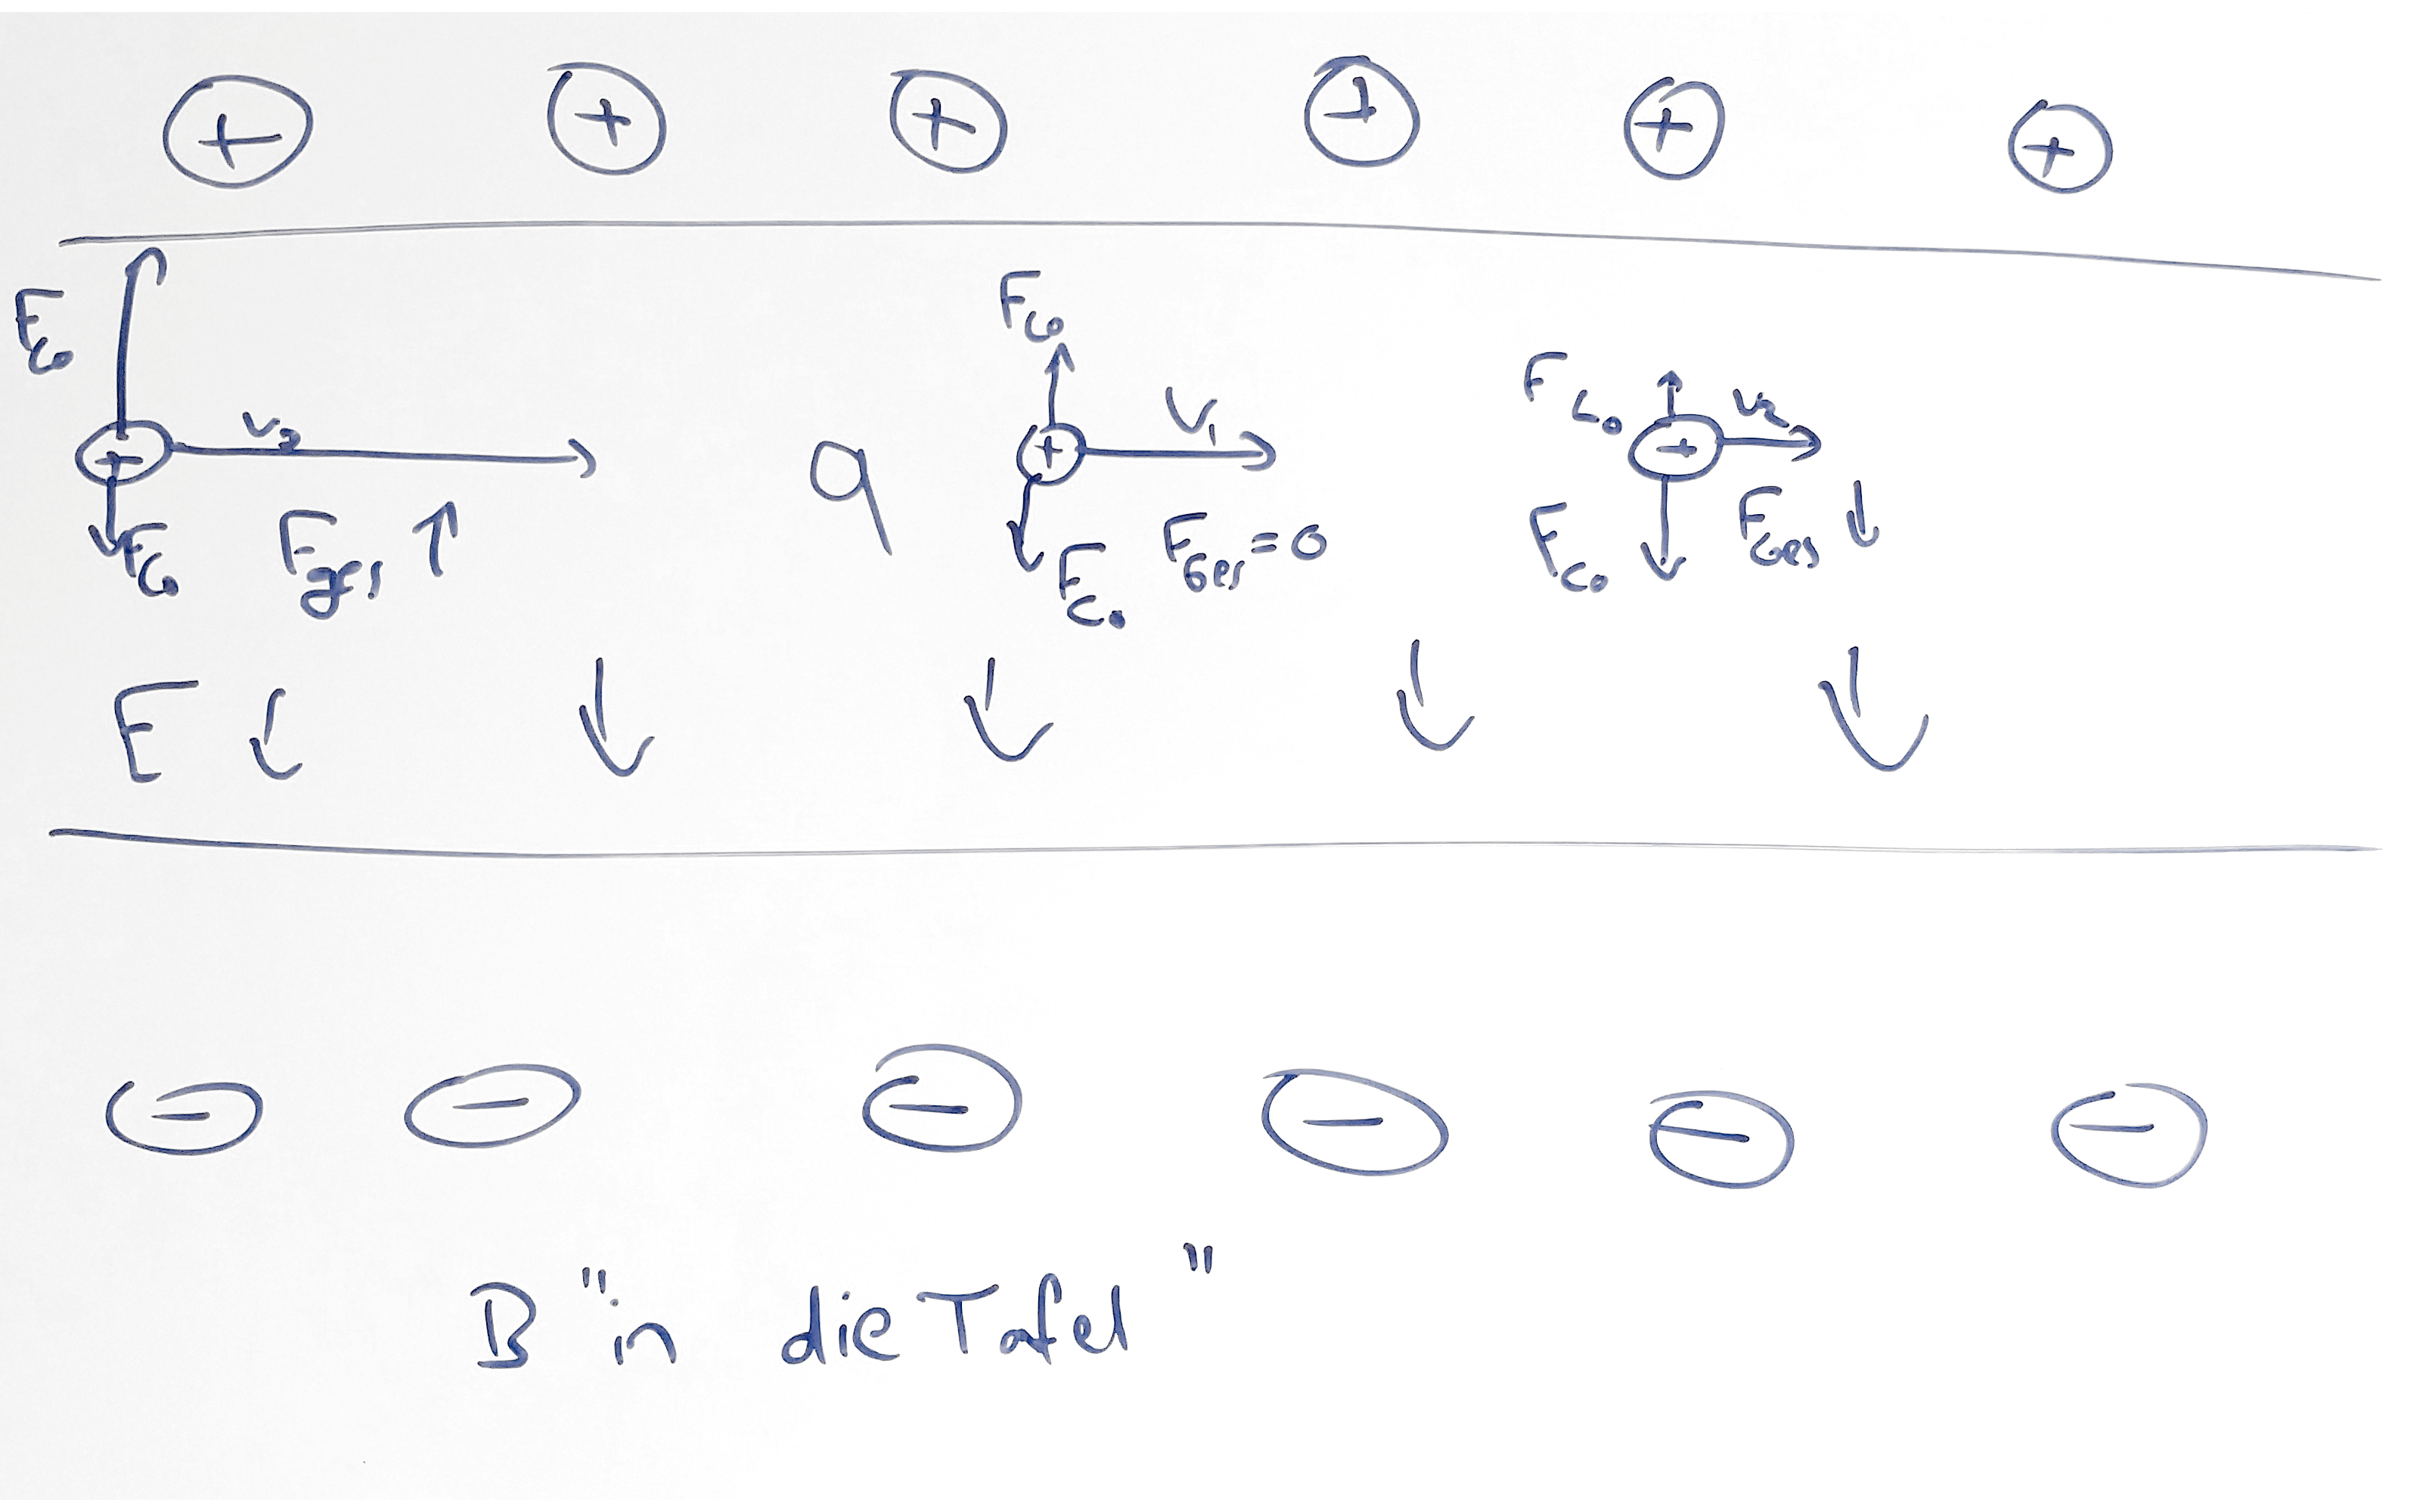
\includegraphics[width=12cm]{aufgabe3a_drift.png}
\end{figure}

\newpage

\vspace{0.5cm}
b) Wenn man den Spalt klein genug macht, so darf die Geschwindigkeit in 
$y$-Richtung nicht stark gewesen sein. Damit können wir die Lorentzkraft 
als konstant annehmen und die auf das Teilchen wirkende Kraft ist 
ebenfalls konstant:
\[ \vec F = q (\vec E + \vec v \times \vec B) = q(E+vB) \cdot \vec e_y \]
Dann können wir für die Koordinaten des Teilchens schreiben ($t_1$ ist 
der Zeitpunkt bei dem das Teilchen den Spalt erreicht):
\begin{align*}
	x(t) &= v\cdot t \Rightarrow t_1 = \frac Lv 
	&
	y(t) &= \frac12 at^2 
	= \frac{q(E+vB)}{2m} t^2 \\ &&
	\Rightarrow
	y(t_1) &= \frac{q(E+vB)}{2m} \frac{L^2}{v^2}
\end{align*}
Wenn der Spalt in $y$-Richtung von $-a$ bis $a$ geht erhalten wir die 
zwei Intervalgrenzen $v_1$ und $v_2$:
\begin{align*}
	% erste geschwindigkeit
	% gleichung aufstellen
	v_1: \quad
	y(t_1) &= \frac{q(E+v_1 B)}{2m} \frac{L^2}{v_1^2} 
	\overset != a \\
	% durch v kuerzen, nach 0 umstellen
	\Rightarrow
	0 &= a - \frac{qEL^2}{2m v_1^2} - \frac{q B L^2}{2m v_1} \\
	% mit v multiplizieren
	&= av_1^2 - \frac{q B L^2}{2m} v_1 - \frac{qEL^2}{2m} \\
	% durch a teilen
	&= v_1^2 - \frac{q B L^2}{2m a} v_1 - \frac{qEL^2}{2m a} \\
	%
	% zweite geschwindigkeit
	% gleichung aufstellebn
	v_2: \quad
	y(t_1) &= \frac{q(E+v_2 B)}{2m} \frac{L^2}{v_2^2} 
	\overset != -a \\
	% durch v kuerzen, nach 0 umstellen
	\Rightarrow
	0 &= a + \frac{qEL^2}{2m v_2^2} + \frac{q B L^2}{2m v_2} \\
	% mit v multiplizieren
	&= av_2^2 + \frac{q B L^2}{2m} v_2 + \frac{qEL^2}{2m} \\
	% durch a teilen
	&= v_2^2 + \frac{q B L^2}{2m a} v_2 + \frac{qEL^2}{2m a} \\
\end{align*}
\newpage
Mit der $pq$-Formel erhalten wir die Lösungen für $v_1$ und $v_2$ (wobei 
der -Teil eine negative Geschwindigkeit erzeugt und ignoriert werden kann)
\begin{align*}
	v_1 &= \frac{q B L^2}{4m a} \pm \sqrt{
		\left(\frac{q B L^2}{4m a}\right)^2 + \frac{qEL^2}{2m a}
	}
	\quad
	&
	v_2 &= -\frac{q B L^2}{4m a} \pm \sqrt{
		\left(\frac{q B L^2}{4m a}\right)^2 - \frac{qEL^2}{2m a}
	}
\end{align*}
	
\vspace{0.5cm}

c) Die Gesamtkraft auf ein geladenes Teilchen im Wienfilter (Summe aus 
Coulomb- und Lorentzkraft) lautet:
\[
	\vec F = q (\vec E + \vec v \times \vec B)
\]
Mit dem 3. Newtonschen Axiom können wir die DGL aufstellen:
\begin{align*}
	\vec F = m \cdot \dot {\vec v} 
	&= q (\vec E + \vec v \times \vec B) \\
	% E feld einsetzen
	&= Eq \ \vec e_y + Bq \ (\dot{\vec v} \times \vec e_z) \\
	% kreuzprodukt ausrechnen
	&= Eq \ \vec e_y + Bq \cdot 
	\begin{pmatrix} v_y \\ -v_x \\ 0 \end{pmatrix} \\
\end{align*}
Man erhält ein System aus 3 Gleichungen:
\begin{align*}
	\dot v_x &= \frac{qB}{m} v_y \tag{3.1}\\
	\dot v_y &= \frac{Eq}{m} - \frac{qB}{m} v_x \tag{3.2}\\
	\dot v_z &= 0 \tag{3.3}
\end{align*}
Durch Ableiten der ersten und einsetzen in die zweite Gleichung bringt uns 
$v_x(t)$:
\begin{align*}
	(3.1) \overset{\frac{d}{dt}}{\Rightarrow}
	\ddot v_x = \frac{qB}{m} \dot v_y \Rightarrow
	\dot v_y &= \frac{m}{qB} \ddot v_x \\
	% einsetzen in 3.2
	\text{Einsetzen in (3.2)} \ \Rightarrow
	\frac{m}{qB} \ddot v_x &=
	\frac{qE}{m} - \frac{qB}{m} v_x \\
	% dgl umstellen
	\ddot v_x + \underbrace{\left(\frac{qB}m \right)^2}_{= \omega^2}
	v_x
	&= \frac{qE}{m} \frac{qB}{m}
\end{align*}
Mit dem Ansatz $v_x(t) = \alpha \sin(\omega t) + \beta \cos(\omega t) + 
\gamma$ erhalten wir mit den Randbedingungen:
\begin{itemize}
	\item $\alpha = 0$, da bei $t=0$ keine Kraft in $x$-Richtung wirkt 
	\item $\gamma$ mit der partikulären Lösung:
	\[ 
		\omega^2 \cdot \gamma = \frac{q^2 \ E \ B}{m^2} 
		\Rightarrow
		\gamma = \frac EB
	\]
	\item $\beta$ folgt aus der Rdb $v_x(0) = v_0$:
	\[
		v_x(0) = \beta \cos(0) + \frac EB = \beta + \frac EB
		\overset{!}{=} v_0
		\Rightarrow
		\beta = v_0 - \frac{E}{B}
	\]
\end{itemize}
Damit lautet die Lösung der $x$-Koordinate:
\[ v_x (t) = \left( v_0 - \frac EB \right) \cos(\omega t) + \frac EB \]

\newpage
Wenn man die Lösung für $v_x$ in (3.2) erhält man durch integrieren eine
Lösung für $v_y$:
\begin{align*}
	\dot v_y &= \frac{Eq}{m} - \frac{qB}{m} v_x \\
	% loesung fue vx einsetzen
	&= \frac{Eq}{m} - \frac{qB}{m} \left(
		\left( v_0 - \frac EB \right) \cos(\omega t) + \frac EB
		\right) \\
	% umstellen fuers kuerzen
	&= \frac{Eq}{m} - \frac{qB}{m} \frac EB  - \frac{qB}{m}\left(
		\left( v_0 - \frac EB \right) \cos(\omega t)
		\right) \\
	% kuerzen
	&= -\frac{qB}{m} \left(v_0 - \frac EB \right)
		\cos (\omega t) \\
	% integrieren um v zu erhalten
	\Rightarrow
	v_y(t)
	&= \frac{-1}{\omega} \frac{qB}{m} \left(v_0 - \frac EB \right)
		\sin (\omega t) \\
	% kuerzen
	&= \left(\frac EB - v_0 \right)
		\sin (\omega t) \\
\end{align*}
Mit $\omega$ als Zyklotron(-kreis-)frequenz
\[ 
	\omega = \frac{qB}{m} 
	\Rightarrow f = \frac{\omega}{2\pi} = \frac{qB}{2\pi m}
\]

\newpage

\section*{Aufgabe 4}

\begin{figure}[H]
	\centering
	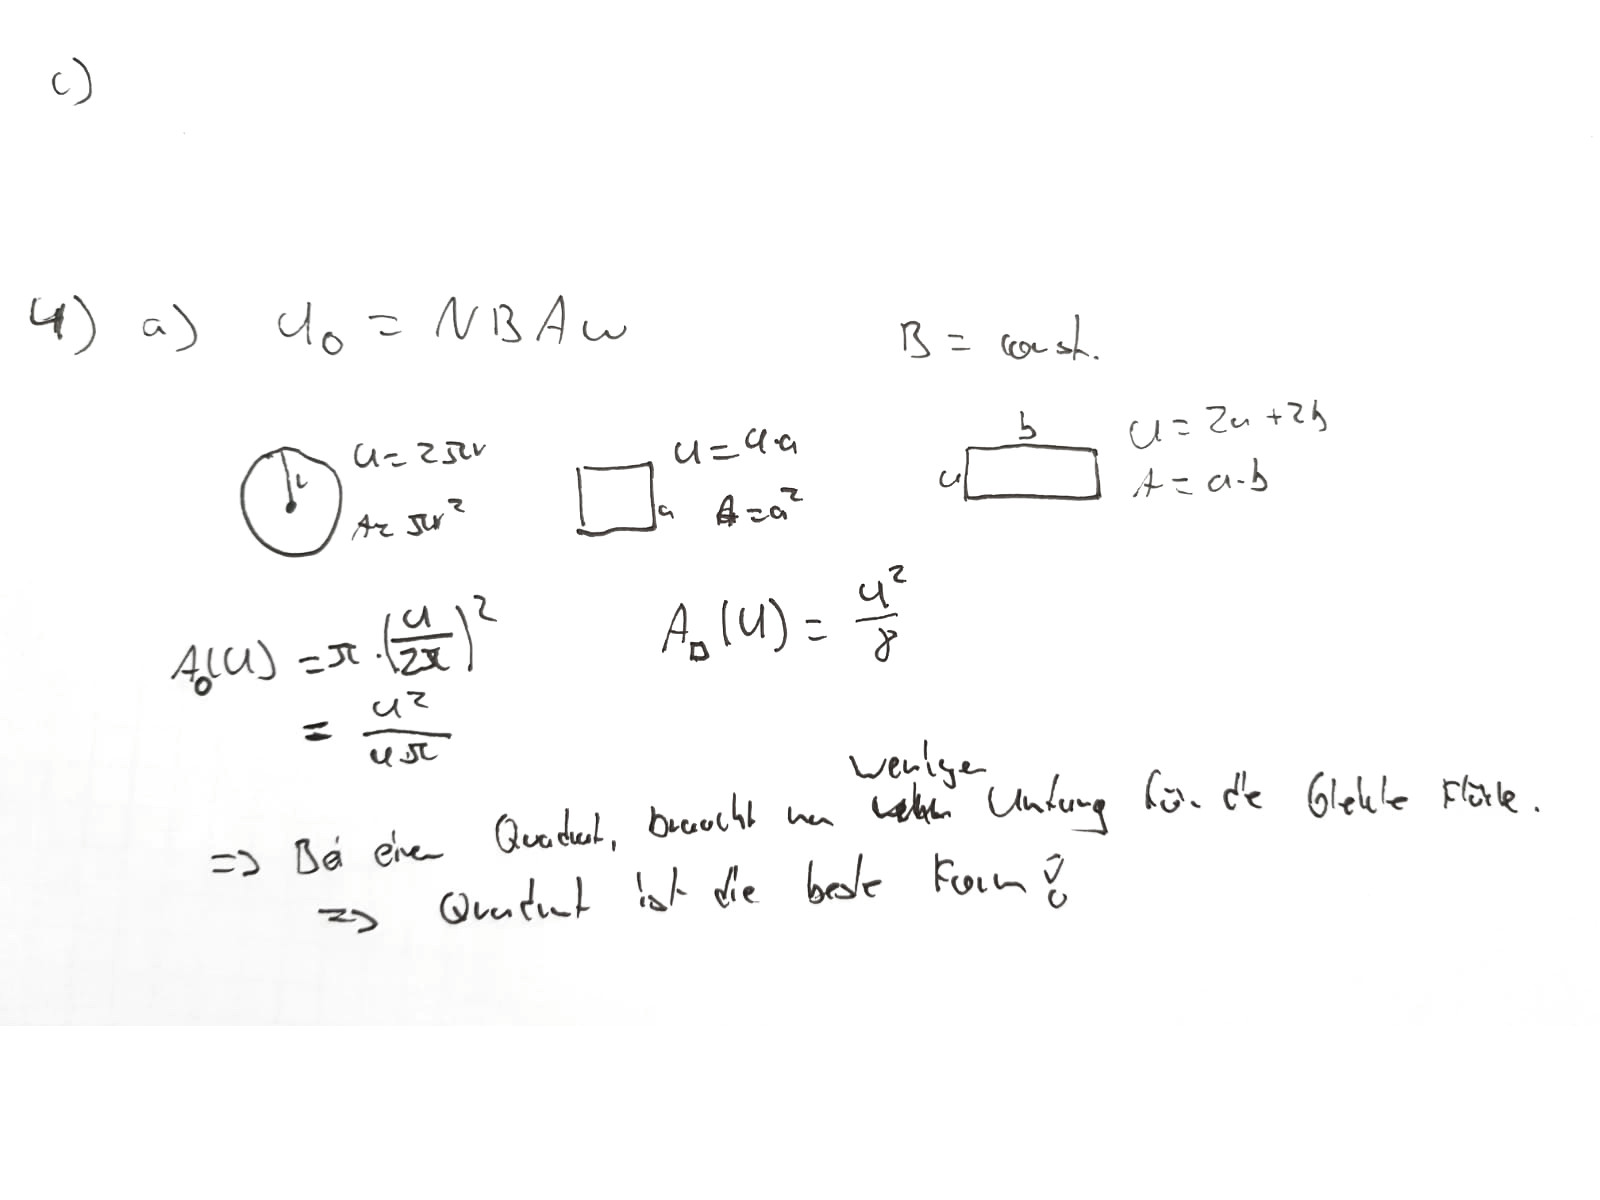
\includegraphics[width=15cm]{4a.jpg}
\end{figure}

\begin{figure}[H]
	\centering
	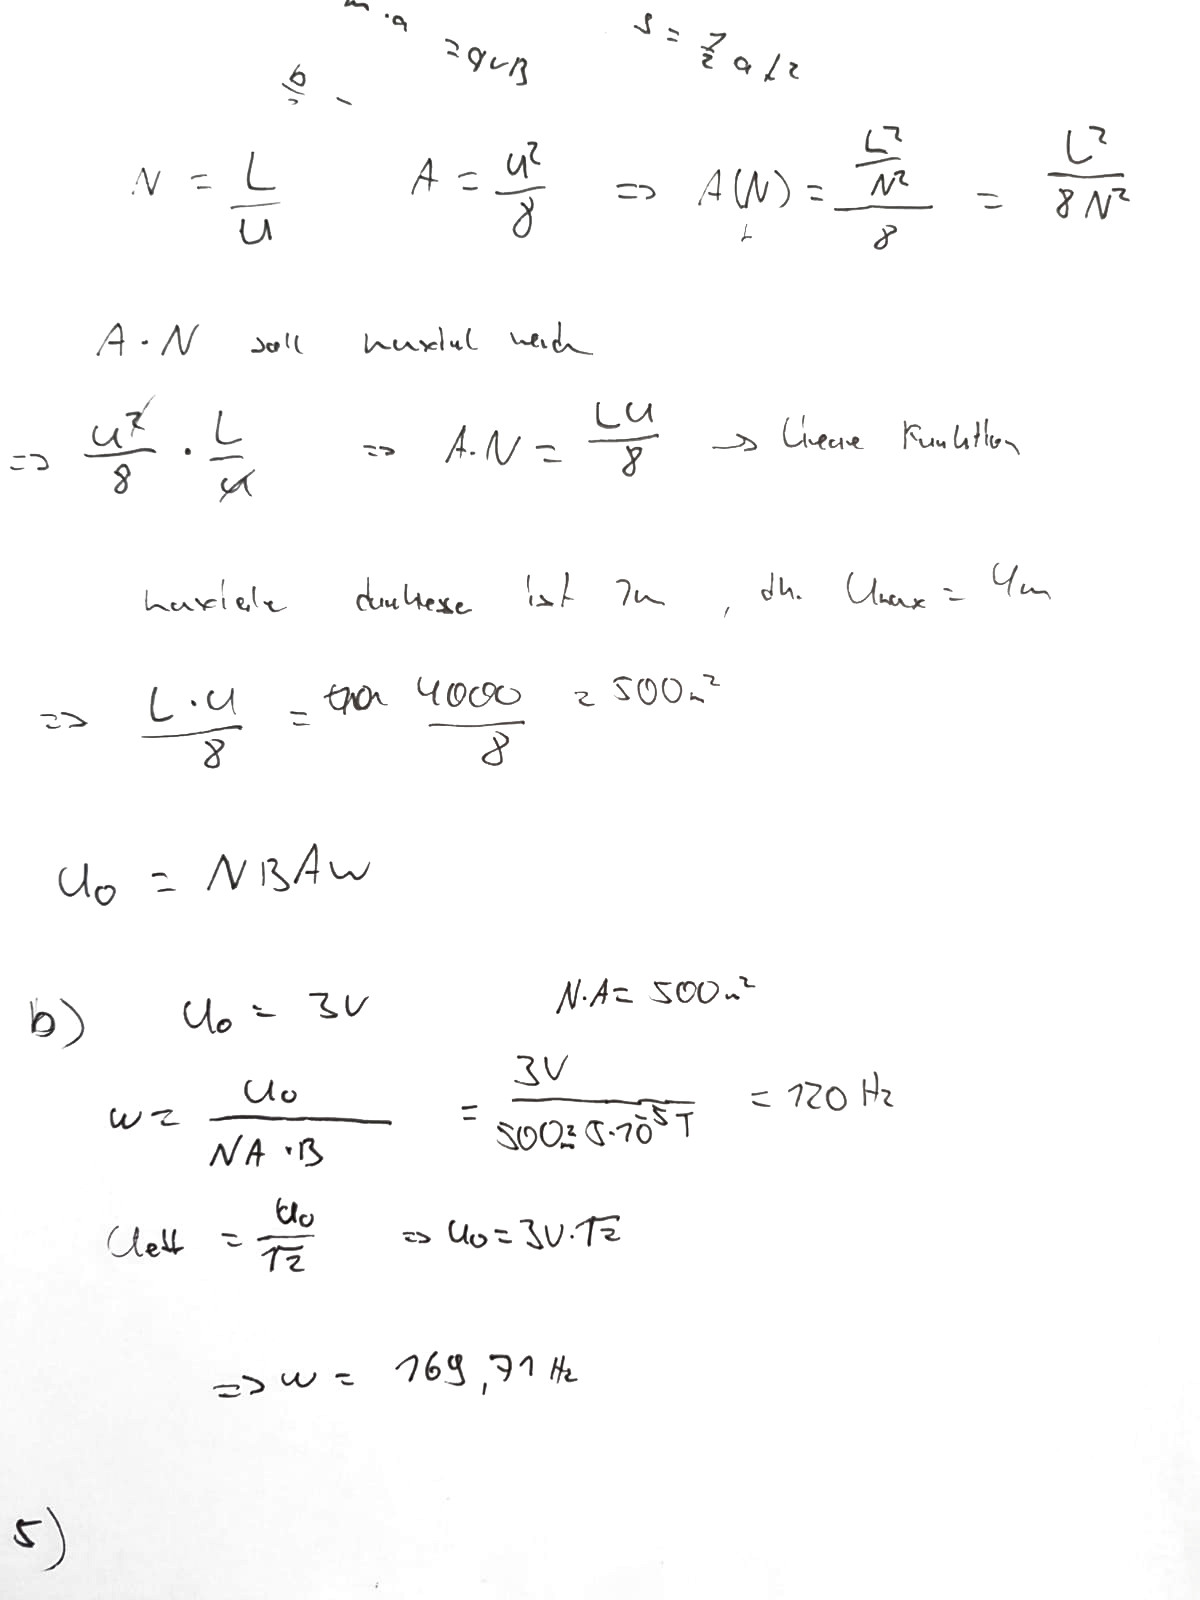
\includegraphics[width=15cm]{4b.jpg}
\end{figure}

\newpage
\section*{Aufgabe 5}

\quad a) Da das $B$-Feld in $z$-Richtung inhomogen ist, verändert sich die 
auch der Magnetische Fluss durch den Ring, wenn er sich in $z$-Richtung
bewegt, da die Feldlinien des externen $B$-Feldes orthogonal auf der
Fläche des Ringes stehen. \\
Der Ring ist eine geschlossene Leiterschleife, d.h. wenn sich der 
magnetische Fluss durch diesen mit der Zeit ändert wird eine
Spannung induziert.\\
Daher ist mit einer Bewegung in $z$-Richtung eine Induktionsspannung
verbunden. \\

Da sich $\vec B_\text{ges}$ aus dem externen Feld ($H$-Feld) und der
Magnetisierung der Luft und des Ringes ($M$-Feld) zusammensetzt,
kann $B_\text{ges} \approx B_\text{ext}$ bei einer geringen Magnetisierung
des Mediums angenommen werden.

\vspace{0.5cm}

b) Die induzierte Spannung hängt direkt mit der Bewegung in $z$-Richtung 
zusammen:
\[
	U_\text{ind} = -\frac{d\Phi_B}{dt}
	= -\frac{d}{dt} A \beta z
	= -A\beta \dot z
\]
Die Gesamtenergie im System setzt sich zusammen aus kinetischer und
potentieller Energie, zusammen mit der Leistung des induzierten Stromes
im Ring (nach der Zeit integriert, die Energie ist in Form von 
thermischer Energie ``verloren``):
\begin{align*}
	E_\text{ges} 
	&= E_\text{kin} + E_\text{pot} + \int_0^t P_\text{ind} \ dt \\
	% P_ind einzetzen
	&= \frac12 mv^2 + mgz 
	+ \int_0^t U_\text{ind} \cdot I_\text{ind} \ dt \\
	% I einsetzen
	&= \frac12 mv^2 + mgz 
	+ \int_0^t \frac{U_\text{ind}^2} R \ dt \\
	% U einsetzen
	&= \frac12 mv^2 + mgz 
	+ \int_0^t \frac{(A\beta \dot z)^2} R \ dt
	\overset != const.
\end{align*}

\vspace{0.5cm}

c) Da $E_\text{ges}$ konstant ist, muss die Ableitung dieser $0$ sein.\\
Dann lässt sich die DGL aufstellen:
\begin{align*}
	\frac{d}{dt} E_\text{ges} 
	= 0
	\overset{!}&{=}
	m v \dot v + mgv
	+ \frac{(A\beta \dot z)^2} R \\
	% dot z ersetzen
	&= m v \dot v + mgv + \frac{(A\beta)^2} R \cdot v^2 \\
	% durch \dot v teilen
	\Leftrightarrow
	0
	&= m \dot v + mg + \frac{(A\beta)^2} R \cdot v \\
	% wie ne dgl hinschrieben
	\Leftrightarrow
	g
	&= - \dot v - \underbrace{\frac{(A\beta)^2}{Rm}}_{\alpha :=}
	\cdot v
\end{align*}
Für die DGL existieren die homogene und partikuläre Lösung:
\begin{align*}
	\text{homogene Lsg:} \ 
	0
	&= - \dot v_h - \alpha v_h
	&
	\text{partikuläre Lsg:} \ 
	g
	&= - \dot v_p - \alpha v_p \\
	% reinigen
	\Leftrightarrow
	0
	&= \dot v_h + \alpha v_h
	&
	\text{Ansatz: } v_p(t) 
	&= \xi_2 \\
	% loesen
	\Rightarrow
	v_h(t) 
	&= \xi_1 \cdot e^{-\alpha t}
	&
	\Leftrightarrow
	g
	&=- \alpha \xi_2 \\
	% v_p loesen
	&&
	\xi_2
	&= -\frac g\alpha
\end{align*}
Unsere allgemein Lösung lautet dann:
\[
	v(t) = v_h(t) + v_p(t) = \xi_1 \cdot e^{-\alpha t} -\frac g\alpha
\]

\newpage

d) Mit unserer Rdb. erhalten wir $v(t)$:
\begin{align*}
	v(0) 
	&= \xi_1 \cdot e^{-\alpha 0} -\frac g\alpha 
	= \xi_1 - \frac g\alpha \overset != 0 \\
	\Rightarrow
	\xi_1 
	&= \frac g\alpha \\
	\Rightarrow
	v(t) 
	&= \frac g\alpha \cdot e^{-\alpha t} -\frac g\alpha
\end{align*}
Damit existiert eine Grenzgeschwindigkeit:
\[
	\lim_{t \rightarrow \infty} v(t)
	=
	\lim_{t \rightarrow \infty}
	\frac g\alpha \cdot e^{-\alpha t} -\frac g\alpha
	=
	-\frac g\alpha
\]




\end{document}
